\documentclass{standalone}
\usepackage{tikz}

\begin{document}

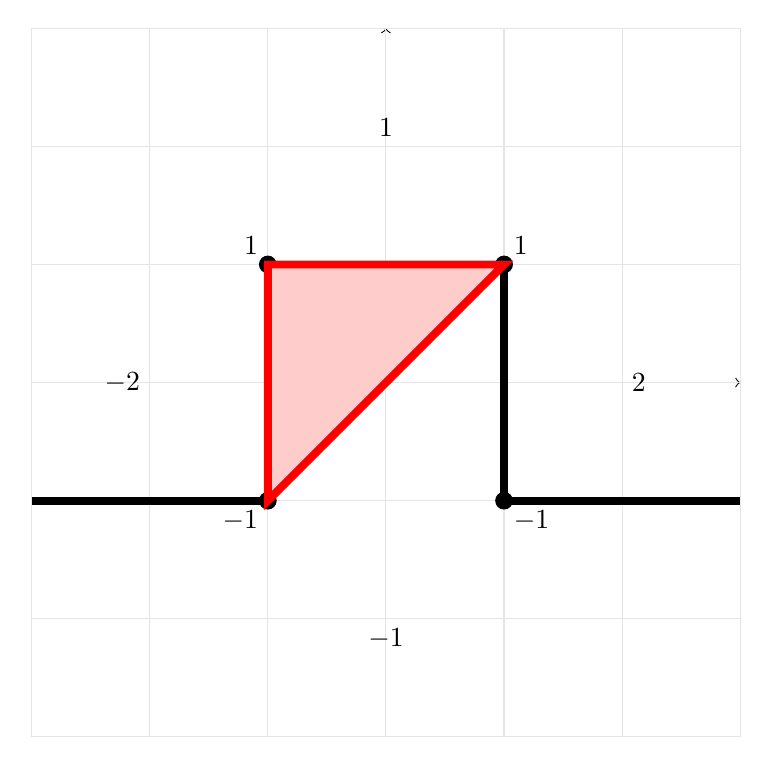
\begin{tikzpicture}[scale=1.5]
    % Draw the axes
    \draw[->] (-3,0) -- (3,0);
    \draw[->] (0,-3) -- (0,3);

    % Draw the grid
    \draw[gray!20] (-3,-3) grid (3,3);

    % Draw the lines
    \draw[line width=1mm] (-3,-1) -- (-1,-1);
    \draw[line width=1mm] (-1,-1) -- (-1,1);
    \draw[line width=1mm] (-1,1) -- (1,1);
    \draw[line width=1mm] (1,1) -- (1,-1);
    \draw[line width=1mm] (1,-1) -- (3,-1);

    % Draw the vertices of the polygon
    \filldraw [black] (-1,-1) circle (2pt);
    \filldraw [black] (-1,1) circle (2pt);
    \filldraw [black] (1,1) circle (2pt);
    \filldraw [black] (1,-1) circle (2pt);

    % Draw the polygon in red
    \draw[red, line width=1mm, fill=red!20] (-1,-1) -- (-1,1) -- (1,1) -- cycle;

    % Label the vertices
    \node at (-1,-1) [below left] {$-1$};
    \node at (-1,1) [above left] {$1$};
    \node at (1,1) [above right] {$1$};
    \node at (1,-1) [below right] {$-1$};

    % Label the axes
    \node at (2,0) [right] {$2$};
    \node at (-2,0) [left] {$-2$};
    \node at (0,2) [above] {$1$};
    \node at (0,-2) [below] {$-1$};
\end{tikzpicture}

\end{document}